\newpage
\begin{slikaDesno}{fig/bouncing_blocks.pdf}
\textbf{{\color{red}*}\ID.}
    У механичком систему са слике познат
је однос 
маса крутих блокова $
\upalpha = \dfrac{M}{m}$. 
Зид са леве је веома масиван и 
практично непокретан, a са десне стране подлога 
се протеже у бесконачност.
Занемарити трење између подлоге 
и блокова, 
$\upmu \to 0$. 
У почетном тренутку су вектори брзина 
блокова
${\bf v} = v_0 {\rm i}_x$ и
${\bf u} = 0$ ($v_0 > 0$). 
\end{slikaDesno}
Након $k$ међусобних судара блокова су 
њихови алгебарски интензитети брзина 
$v[k]$ и $u[k]$.
% Нацртати (а) 
% блок дијаграм система, без улаза, 
% користећи идеалне блокове за кашњење, сабираче
% и множаче, тако да су његови излази буду 
% $v[n]$ 
% и $u[n]$, 
% барем до тренутка када 
% више нема судара у систему. 
(а) Одредити низове $v[k]$ и $u[k]$.
Одредити (б) укупан
број судара између блокова у процесу, $N$, 
ако је $\upalpha = 400^m$, где је $m$ цео број.
Сматрати да су сви судари у систему 
\textit{апсолутно еластични}. 

\textit{\myul{Помоћ}}. Након 
апсолутно еластичног
судара, дуж правца, између блокова масе $m_1$ и $m_2$ 
почетних алгебарских интензитета брзина $u_1$ и 
$u_2$ њихови нови алгебарски интензитети брзина су 
$v_1 = \dfrac{m_1-m_2}{m_1+m_2} u_1 + 
\dfrac{2m_2}{m_1+m_2} u_2$  и 
$v_2 = 
\dfrac{2 m_1}{m_1+m_2} u_1
+
\dfrac{m_2 - m_1}{m_1 + m_2} u_2  
$ редом. Референтни смерови брзина блокова 
су \myul{један ка другом}. \\

\textsc{\underline{Решење}}: Пошто се судари дешавају у дискретним временским тренуцима 
док је између њих стање система непроменљиво, процес представљен у задатку се може сматрати
\textit{дискретним} у односу на текући број судара. Стање након $k$-тог судара описано је
системом датих диференцних једначина као 
\begin{eqnarray}
    v[k+1] & = & \dfrac{M - m}{M + m} v[k] + \dfrac{2m}{M + m} (-u[k]) \\[2mm]
    u[k+1] & = & \dfrac{2M}{M + m} v[k] + \dfrac{m - M}{M + m} (-u[k]),
\end{eqnarray} 
Важно је нагласити да се у једначинама појављује $-u[k]$ будући да леви блок у судару учествује 
\textit{након} одбијања о зид са леве стране што доводи до промене знака брзине тог блока. 
Елиминисањем конкретних маса преко задатог параметра $\upalpha$ има се
\begin{eqnarray}
    v[k+1] & = & \dfrac{\upalpha - 1}{\upalpha + 1} v[k] - \dfrac{2}{\upalpha + 1} u[k] \\[2mm]
    u[k+1] & = & \dfrac{2\upalpha}{\upalpha + 1} v[k] - \dfrac{1 - \upalpha}{\upalpha + 1} u[k]
\end{eqnarray} 

%(а)

(б) Одређивање одзива система обавља се применом $\mathcal{Z}$-трансформације уз уважавање почетних 
услова\footnote{Користи се теорема $\mathcal Z\{x[n + 1]\} = z(\mathcal Z \{x[n]\} - x[0])$. }
чиме се добија
\begin{eqnarray}
    z(V(z) - 
    \cancelto{v_0}{v[0]}
    ) & = & \dfrac{\upalpha - 1}{\upalpha + 1} V(z) - \dfrac{2}{\upalpha + 1} U(z) \\[2mm]
    z(U(z) - \cancel{u[0]} ) & = & \dfrac{2\upalpha}{\upalpha + 1} V(z) - \dfrac{1 - \upalpha}{\upalpha + 1} U(z)
\end{eqnarray}
Сређивањем израза у форму система алгебарских једначина по $V(z)$ и $U(z)$ има се.
\begin{eqnarray}
    - z v[0] & = & \left( \dfrac{\upalpha - 1}{\upalpha + 1} - z \right) V(z) - \dfrac{2}{\upalpha + 1} U(z) \\[2mm]
    0 & = & \dfrac{2\upalpha}{\upalpha + 1} V(z) - \left( \dfrac{1 - \upalpha}{\upalpha + 1} + z \right) 
    U(z)
\end{eqnarray}
Решавањем система једначина налазе се резултати: 
\begin{eqnarray}
    U(z) & = & 
    \frac{2 \alpha v_{0} z}
    {z^{2} + 2 z \dfrac{1 - \upalpha}{1 + \upalpha} + 1}
    \\[2mm]
    V(z) & = & 
    \frac{v_{0} z \left(z + \dfrac{1 - \upalpha}{1 + \upalpha} \right) }
    {z^{2} + 2 z \dfrac{1 - \upalpha}{1 + \upalpha} + 1}
\end{eqnarray}
Непосредном идентификацијом, одређујемо инверзну $\mathcal{Z}$-трансформацију добијених резултата: 
$u[k] = v_0\sqrt\upalpha \sin(k\Upomega_0)$ и 
$v[k] = v_0\cos(k\Upomega_0)$, где је $\Upomega_0 = \arccos\left( \dfrac{\upalpha-1}{\upalpha+1} \right)$.

\begin{figure}[b!]
    \centering
    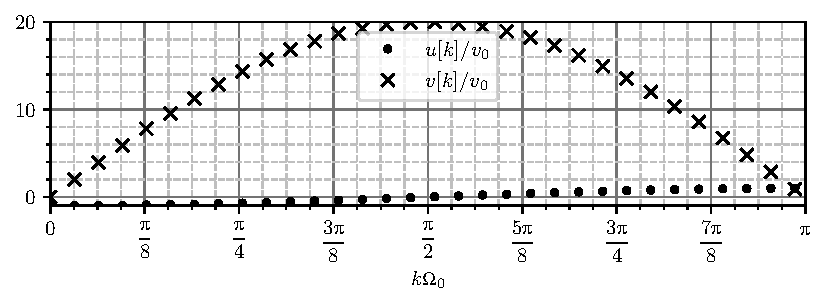
\includegraphics[scale=1]{fig/blokovi_plot.pdf}
    \caption{Пример за $\upalpha = 400$, укупно $N = \lfloor 10\uppi \rfloor = 31$ судара.}
    \label{fig:\ID.primer}
\end{figure}

Блокови ће наставити сударање све док након $k$ судара брзина десног блока у десно не постане
већа од брзине левог блока -- односно, када након одбијања левог блока о зид он не буде могао да 
сустигне већи блок. То је изражено условом у облику $- v[k] \geq u[k]$.  Гранично решење потражимо
у скупу реалних бројева сменом $k \mapsto t$ као
\begin{eqnarray}
    - \cancel{v_0} \cos(t\Upomega_0) & = & \cancel{v_0} \sqrt{\upalpha} \sin(t\Upomega_0)
    \Rightarrow
    \cos(t\Upomega_0) = -\sqrt{\upalpha} \sin(t\Upomega_0) \Rightarrow 
    \tan(t\Upomega_0) = -\dfrac{1}{\sqrt{\upalpha}}
    \\
    & \Rightarrow & t = \dfrac{1}{\Upomega_0} 
    \left( \arctan\left(-\dfrac1{\sqrt{\upalpha}} \right) + \uppi \right)
    \\
    & \Rightarrow & k_\mr{max} = N = \lfloor t \rfloor = \left\lfloor \dfrac{1}{\Upomega_0} \left( \arctan\left(
        -\dfrac1{\sqrt{\upalpha}} \right) + \uppi \right) \right\rfloor
        \label{eq:\ID.collisions}
\end{eqnarray}

Размотримо шта се дешава када $\upalpha$ постаје велико. Тада је 
$\arctan \left(- \dfrac1{\sqrt{\upalpha}} \right) 
\to 0$, a добијена дискретна кружна учестаност се може апроксимирати у околини јединице
помоћу Тејлоровог развоја\footnote{Када је $x\to 0$ тада је $\arccos(1 - x) \approx \sqrt{2x}$} поступком
\begin{equation}
    \Upomega_0 = \arccos\left( \dfrac{\upalpha-1}{\upalpha+1} \right)
    = \arccos\left( 1 - \dfrac{2}{\upalpha+1} \right)
    \approx \dfrac{2}{\sqrt{ \upalpha }}
\end{equation}
Заменом добијене апроксимације у израз \ref{eq:\ID.collisions} добија се резултат:
$N = \left\lfloor \uppi \sqrt{\upalpha}/2 \right\rfloor$. \vspace{1mm} 
Односно, уколико је $\upalpha = 400^m$ онда је 
$N = \left\lfloor 10^m \uppi \right\rfloor$, дакле, првих $m$ цифара броја $\uppi$ (!)
На слици \ref{fig:\ID.primer} приказан је један пример сигнала $v[k]$ и $u[k]$ за 
$\upalpha = 400$. 
